\documentclass{article}
\usepackage[T1]{fontenc}
\usepackage[utf8]{inputenc}
\usepackage{amsmath}
\usepackage{amssymb}
\usepackage{tikz}
\usetikzlibrary{automata,positioning}

\title{Proof: The Reverse of a Regular Language is Regular}
\author{Tanisha Ahuja \and Natasha}
\date{\today}

\begin{document}
\maketitle

\section{Problem Statement}
For any DFA $M$, prove that the reverse of strings in $L(M)$, that is $(L(M))^R = \{ w^R \mid w \in L(M) \}$, is regular.

\section{Proof Strategy}
We will prove this by construction. Given a DFA $M$, we will:
\begin{enumerate}
    \item Convert $M$ to an NFA $M'$ that accepts the reverse language
    \item Show that $M'$ is a valid NFA
    \item Since NFAs recognize regular languages, this proves $(L(M))^R$ is regular
\end{enumerate}

\section{Construction}
Given a DFA $M = (Q, \Sigma, \delta, q_0, F)$, we construct an NFA $M' = (Q, \Sigma, \delta', F, \{q_0\})$ where:
\begin{itemize}
    \item The states $Q$ remain the same
    \item The alphabet $\Sigma$ remains the same
    \item The transition function $\delta'$ is reversed: for each transition $\delta(q,a) = p$ in $M$, 
          we add a transition $\delta'(p,a) = q$ in $M'$
    \item The start state of $M$ becomes the only accepting state in $M'$
    \item The accepting states $F$ of $M$ become the start states in $M'$
\end{itemize}

\section{Proof of Correctness}
Let $w = a_1a_2...a_n$ be a string in $L(M)$. Then there exists a sequence of states 
$r_0,r_1,...,r_n$ in $M$ where:
\begin{itemize}
    \item $r_0 = q_0$
    \item $\delta(r_i,a_{i+1}) = r_{i+1}$ for $0 \leq i < n$
    \item $r_n \in F$
\end{itemize}

In $M'$, we can follow the reverse path for $w^R = a_n...a_2a_1$:
\begin{itemize}
    \item Start from $r_n$ (which is a start state in $M'$)
    \item Follow reversed transitions
    \item End at $r_0$ (which is the accepting state in $M'$)
\end{itemize}

Therefore, $w^R$ is accepted by $M'$ if and only if $w$ is accepted by $M$.

\section{Example}
\begin{center}
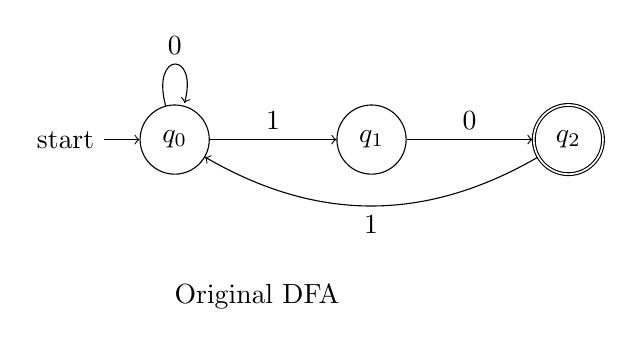
\begin{tikzpicture}[auto,node distance=2.5cm]
    % Original DFA
    \node[state,initial] (q0) {$q_0$};
    \node[state,right of=q0] (q1) {$q_1$};
    \node[state,accepting,right of=q1] (q2) {$q_2$};
    
    \path[->]
        (q0) edge[loop above] node{0} (q0)
        (q0) edge[above] node{1} (q1)
        (q1) edge[above] node{0} (q2)
        (q2) edge[bend left] node{1} (q0);
    
    \node[text width=3cm] at (1.5,-2) {Original DFA};
\end{tikzpicture}

\vspace{2cm}

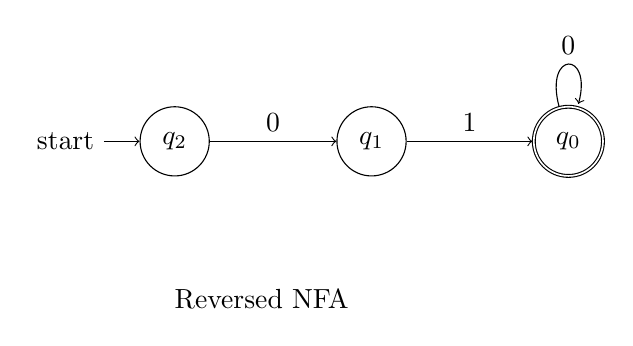
\begin{tikzpicture}[auto,node distance=2.5cm]
    % Reversed NFA
    \node[state,initial] (q2) {$q_2$};
    \node[state,right of=q2] (q1) {$q_1$};
    \node[state,accepting,right of=q1] (q0) {$q_0$};
    
    \path[->]
        (q2) edge[above] node{0} (q1)
        (q1) edge[above] node{1} (q0)
        (q0) edge[loop above] node{0} (q0);
    
    \node[text width=3cm] at (1.5,-2) {Reversed NFA};
\end{tikzpicture}
\end{center}

\end{document}